\section{DISE\~NO EXPERIMENTAL}

El objetivo de este capítulo es presentar los aspectos del experimento y la forma como se llevó a cabo a cabo con la finalidad de validar científicamente la efectividad del \textit{meetingware} D-Minute. Este \textit{groupware} es un medio para generar reuniones de trabajo que apostamos que ahorran tiempo y harán hacer circular el conocimiento de mejor manera que las actas que se toman de la manera tradicional. Sin embargo, para ello es preciso definir el diseño experimento para probar esas características. En primer lugar, se establece la variables experimentales del fenómeno. Más adelante, se describen las características de las prueba científica y en forma posterior se presenta el protocolo de la investigación. Por último, se entrega el resumen del contenido del capítulo. 

\subsection{INVESTIGACIÓN CIENTÍFICA}

Con el objetivo de establecer el marco científico que orienta la investigación del presente trabajo, se expone mediante pregunta el problema a resolver de la cual se deriva las hipótesis que se requiere comprobar en este estudio.

\subsubsection{Pregunta}

Las preguntas que guía este estudio y fueron presentadas en el capítulo 1  se expone a continuación para que la investigación sea expresada en toda su dimensión contextual.\newline

\textbf{PREGUNTA 1:} ¿Cómo mostrar la efectividad de un \textit{meetingware} basado en una teoría del diálogo, D-Minute, versus la adopción de actas de reuniones manejadas con ofimática tradicional?\newline

\textbf{PREGUNTA 2:} ¿Cómo saber si la percepción de la circulación del conocimiento de los actores del \textit{meetingware} propuesto, D-Minute, supera a las de las actas tradicionales manejadas con ofimatica?

\subsubsection{Variable}

Tras expuesta las preguntas de investigación es importante mencionar cómo se construye la hipótesis de este estudio y para ello se describen en primer lugar  las siguientes variables del estudio: 

\begin{enumerate}[1.]
    \item \textbf{Independientes} (Causa): Se definen dos tratamientos para determinar el manejo de la memoria en las reuniones: 
    \begin{enumerate}[a.]
	    \item Actas en papel hechas de manera \textit{ad-hoc}. 
		\item Sistema tecnológico “D-Minute”.
    \end{enumerate}

    \item \textbf{Dependientes} (Efecto): Cada tratamiento generará un efecto que necesita ser medido de forma cualitativa y cuantitativa. Se consideran dos factores como parte del efecto:
    \begin{enumerate}[a.]
	    \item \textbf{Circulación del conocimiento} que posee la herramienta para recuperar el contexto de las reuniones pasadas, medible de forma cuantitativa por medio de un cuestionario.
	    \item \textbf{Tiempo} que requieren los participantes para retomar los elementos del diálogo, medible de forma cualitativa dado que se debe analizar, con el fin de calcular el tiempo que implica retomar los elemento del diálogo en las reuniones experimento.
    \end{enumerate}

    \item \textbf{Controladas}: Dichas variables serán relevantes a la hora de ejecutar el experimento con el fin de que cada grupo pueda operar en igualdad de condiciones:
    \begin{enumerate}[a.]
	    \item Grupos de 7 personas, heterogéneo.
	    \item El grupo tenga el mismo nivel educacional (pregrado o postgrado) y habilidades técnicas similares o complementables.
	    \item El rango de edad del grupo reclutados debe estar dentro de los 27 a 45 años.
	    \item Las personas del experimento tienen experiencia con proyectos que utilicen alguna metodología de desarrollo de \textit{software} tradicional
	    \item El nivel de complejidad del proyecto a abordar sea bajo y el tiempo de desarrollo sea de dos a tres meses.
	    \item El espacio físico para llevar a cabo la reunión tendrá las condiciones necesarias para una correcta y cómoda ejecución de las reuniones-experimento.
	    \item Los tratamientos deberán ser expuestos por el líder de la reunión por medio de un \textit{datashow} o pizarra electrónica o pantalla gigante conectado al \textit{notebook} de la reunión y que siempre está a la vista de los participantes de la reunión.
    \end{enumerate}

\end{enumerate}

\subsubsection{Hipótesis}

A partir de la pregunta de investigación y las variables del estudio - descritas anteriormente - se desprenden las siguientes hipótesis:

\begin{enumerate}[1.]
	\item $\mathrm{H_{Tiempo}}$: Las personas mediante el uso de D-Minute pueden restablecer el hilo conversacional de las reuniones pasadas y el estado de las tareas en un menor tiempo que utilizando minutas tradicionales realizadas con tecnologías de ofimática genéricas.
	\item $\mathrm{H_{Conocimiento}}$: En relación a las actas de reuniones que usan ofimática, D-Minute permite hacer circular el conocimiento de mejor manera según la percepción de los miembros del equipo de proyecto.
\end{enumerate}

Esta segunda hipótesis está basada en los conceptos de \textit{knowledge management} \fullcite{RN26} considerado en el diseño del \textit{meetingware} D-minute. Además, en esta herramienta se adoptan los conceptos de los elementos del diálogo y el uso de tableros \textit{kanban} para realizar tareas que se coordinan de reunión en reunión, ver capítulo 2 sección 2.2.

\subsection{CARACTERÍSTICA DE LA PRUEBA CIENTÍFICA }

La hipótesis de este trabajo requiere un \textit{test} de significatividad estadística que comúnmente son usados en investigación empírica. La hipótesis considera las siguientes características:

\begin{enumerate}[1.]
	\item \textbf{Validez interna}: no se generaliza a todos los grupos de trabajo puesto que es válido solo para la muestra.
	\item \textbf{Criterios similares}: implica que los grupos operan con características similares en base a criterios objetivos, para que los resultados sean comparables.
	\item \textbf{Exploratorio}: que implica no llegar al mínimo de muestras necesarias para una significancia estadística.

\end{enumerate}

\subsection{PROCEDIMIENTO EXPERIMENTAL}

A continuación, se detalla el protocolo que será utilizado en la investigación. Siendo el encargado de la realización del experimento el estudiante de Magister - que escribe esta propuesta - el cual será supervisado por el Doctor Edmundo P. Leiva Lobos:

\subsubsection{Participante y reclutamiento}

Los sujetos, deberán ser trabajadores de una empresa a elección que pertenezcan a un área de negocio o informática, su rango de edad estará entre los 24 a los 45 años, con un nivel educacional equivalente a formación profesional. El número total de sujetos a considerar en esta investigación es de 14, que se desglosan en dos grupos: grupo de control con 7 sujetos y grupo experimental con 7 sujetos.

\subsubsection{Estímulo y tratamiento}

En el experimento se debe establecer diferencias significativas entre grupo de control y el experimental. Para esto, se administrará un “\textit{coaching}” sobre el diálogo a ambos grupos; pero se espera que los que utilicen D-Minute tengan mejores efectos en las variables dependientes que se van a medir. Además, a ambos grupos (control y experimental) se les imprimirá una ayuda de memoria que explique claramente y sin ambigüedad que significa los elementos del diálogo "co, ac, du, de" y las tareas “ta”. En otras palabras, se les dará un tríptico donde se defina que es un acuerdo, un compromiso, una duda y un desacuerdo; incluyendo como dirimir confusiones comunes sobre estos términos y que las personas comúnmente tienen en el lenguaje coloquial. La idea es que las personas que participan del experimento también tomen conciencia de los actos del habla \fullcite{RN18} que usan en las reuniones.

\subsubsection{Configuración de experimentación}

La experienciase realizará en dependencias de la empresa seleccionada o en la Universidad, en Santiago de Chile. La manera en que se realizará la toma de las muestras será:

\begin{enumerate}[1.]
	\item Preparación del ambiente reunión tras reunión, ver imagen \ref{img5-1}
	\item Grabación en voz del desarrollo de la reunión 
	\item Grabación de vídeo del desarrollo de la reunión
	\item La grabación de la interacción del sujeto con la aplicación D-Minute, mediante algún \textit{software} que capture la actividad del líder de la reunión manipulando D-Minute mientras se efectúa la reunión con el \textit{datashow}
	\item Al finalizar las 4 sesiones de la investigación, realizar encuesta KNA desarrollada por \fullcite{RN36}, indicada en anexo B
\end{enumerate}

Para el grupo de control, sólo se les indicará que deben usar actas en papel del tipo \textit{ad-hoc} o bien utilizar las herramientas genéricas que comúnmente se usa en ofimática como MS-Word. La idea es que se adopte una forma alternativa a D-Minute para confeccionar las minutas de reuniones de trabajo, utilizando si las personas lo desean los elementos de diálogo explicados en el \textit{coaching} administrado.

\begin{figure}[h]
\centering
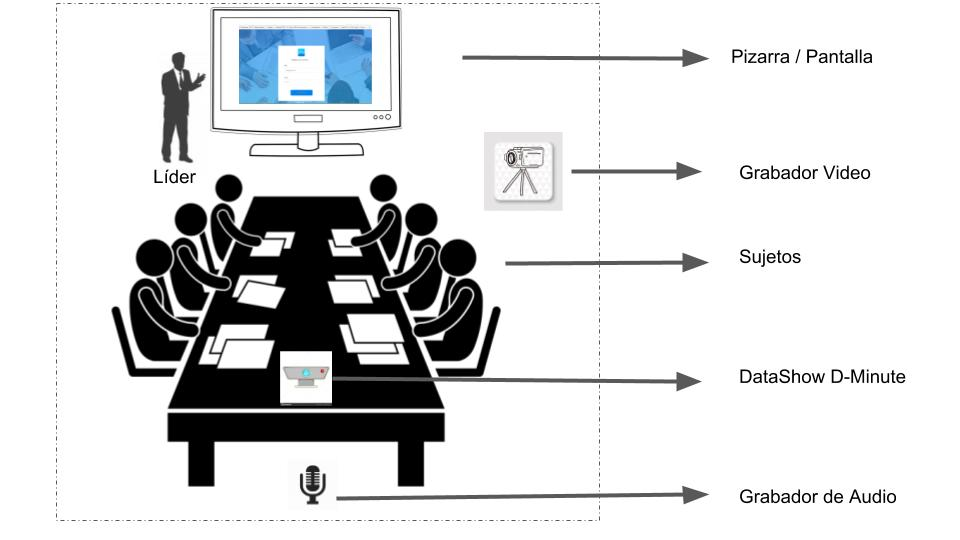
\includegraphics[width=0.8\linewidth]{/setting}
\caption{\textit{Setting} del experimento,  elaboración propia} 
\label{img5-1}
\end{figure}

\subsubsection{Aparato, \textit{software} e instrumento}

Para la captura de datos se requieren instrumentos que nos permitan grabar las sesiones durante el experimento como también el audio de las conversaciones generadas. Ambos en forma separada y con instrumentos diferentes a fin de no perder la calidad para futuros trabajos. 

Otros \textit{software} importantes a considerar es un mezclador de video y voz para unir los datos que se van a capturar de forma separada como también un \textit{software} de transcripción de voz para detectar los actores participantes.

Con el fin de evaluar la circulación de conocimiento se debe utilizar una encuesta del tipo checklist obtenido desde \textit{Knowledge Creation Approach} \fullcite{RN36}. Los resultados serán evaluados en una escala de \textit{Likert}, ver anexo B.

Por último, se requiere de un \textit{notebook} con características básicas para proyectar el \textit{software} de reuniones (D-Minute) del grupo experimental y otro para el grupo de control (actas ofimática) y un proyector. Con las siguientes características recomendadas:

\begin{enumerate}[1.]
	\item Procesador Intel(R) Core 1.3, o superiores
	\item Memoria RAM 4 GB o con mayor capacidad
	\item Disco Duro de 250GB o con 100MB de espacio libre
	\item Tener instalado Java(TM) SE \textit{Runtime Environment} versión 1.8 o superior
	\item Por lo menos una entrada USB 2.0 o mayor
	\item Por lo menos un puerto HDMI

\end{enumerate}

\begin{table}[!h]
\centering
\caption{Alternativas de productos para captura de audio, elaboración propia}
\label{tab:prod31}
\resizebox{15cm}{!} {
\begin{tabular}{|l|c|l|}
\hline
\multicolumn{1}{|c|}{Producto} & \multicolumn{1}{c|}{Precio} & \multicolumn{1}{c|}{URL} \\ \hline
Sennheiser e614 & 219.900 pesos & \url{http://www.centralmusic.cl/microfonos-de-condensador/522-sennheiser-e614-microfono-condensador} \\ \hline
Sennheiser mk8 mic & 609.900 pesos & \url{http://www.centralmusic.cl/microfonos-de-condensador/2939-sennheiser-mk8-mic-condensador} \\ \hline
Rode NT-USB Micrófono Condensador & 149.900 pesos & \url{http://www.centralmusic.cl/microfonos-usb/3348-rode-nt-usb-microfono-condensador} \\ \hline
Voice Tracer DVT7000 (Phillips) & 129 dolares & \url{https://www.philips.com.mx/c-p/DVT7000_00/voice-tracer-captacion-de-sonido-en-360degree} \\ \hline
Business Recorder & 2.990 dólares & \url{http://www.meste.cl/Grabacion_de_Voz/Productos/Grabacion/Business_Recorder___Sala_de_Reuniones/} \\ \hline
Tascam DR 05 & 117.810 pesos & \url{http://davidandjoseph.cl/djcl/tascam-dr-05-grabador-de-audio-portatil} \\ \hline
\end{tabular}
}
\end{table}

\begin{table}[!h]
\centering
\caption{Alternativas de productos para transcribir audio, elaboración propia}
\label{tab:prod2}
\resizebox{15cm}{!} {
\begin{tabular}{|l|c|l|}
\hline
\multicolumn{1}{|c|}{Producto} & \multicolumn{1}{c|}{Precio} & \multicolumn{1}{c|}{URL} \\ \hline
Dragon & 399 euros & \url{https://www.nuance.com/es-es/dragon/transcription-solutions.html} \\ \hline
Trascribe & 20 dolares/año & \url{https://transcribe.wreally.com/account/license/purchase} \\ \hline
\end{tabular}
}
\end{table}

\begin{table}[!h]
\centering
\caption{Alternativas de productos para proyectar video, elaboración propia}
\label{tab:prod3}
\resizebox{15cm}{!} {
\begin{tabular}{|l|c|l|}
\hline
\multicolumn{1}{|c|}{Producto} & \multicolumn{1}{c|}{Precio} & \multicolumn{1}{c|}{URL} \\ \hline
Proyector Nebula & 399.990 pesos & \url{https://ankerstore.cl/proyector-smart-pocket-cinema-nebula-capsule-by-anker?gclid=CjwKCAjw_IPcBRAjEiwAl44QkV-pQoIhQBSny8LK-l9ZFOz0f-HbdhTwqev7sHL9rbWcAmpKSdAO5hoCFUUQAvD_BwE} \\ \hline
Proyector LG & 344.000 pesos & \url{https://www.ebay.com/itm/LG-PH550-Minibeam-LED-Pico-Portable-Projector-with-Built-in-Battery} \\ \hline
\end{tabular}
}
\end{table}

\begin{table}[!h]
\centering
\caption{Alternativas de productos para la captura de video, elaboración propia}
\label{tab:prod4}
\resizebox{15cm}{!} {
\begin{tabular}{|l|c|l|}
\hline
\multicolumn{1}{|c|}{Producto} & \multicolumn{1}{c|}{Precio} & \multicolumn{1}{c|}{URL} \\ \hline
Grabadora Sony & 150.000 pesos & \url{https://store.sony.cl/hdr-cx405/p?idsku=165&utm_source=GooglePLA&sem-la-nb-ss-070218-cl-shopping&gclid=CjwKCAjwrNjcBRA3EiwAIIOvq6_oX5J9igQJ-RzC4BClujEEM2AkQoXZi1Vs4ZV_d9oKafoHvqeNARoC7-UQAvD_BwE} \\ \hline
Grabadora Handycam & 172.000 pesos & \url{http://www.audiomusica.com/catalogo/grabadora-de-video-digital-handycam-q4.html?gclid=CjwKCAjwrNjcBRA3EiwAIIOvq9ZZLl9R9q_CUU7KrQMiQW7vFJxfyDr6ydbuVBzGeNqNEOgVEG7A5xoClr0QAvD_BwE} \\ \hline
\end{tabular}
}
\end{table}

\subsubsection{Procedimiento concreto y aplicación de tarea}

El experimento consiste en trabajar en un proyecto que una vez a la semana y durante cuatro sesiones corridas se revise el avance para dilucidar su estado y a la vez su seguimiento, incluye su planificación futura. Cada tratamiento utilizara un tipo específico de acta. El grupo experimental utilizara el sistema D-Minute y el grupo de control actas en ofimática (versión\textit{ad-hoc}) de forma tal que sea posible observar la recuperación del hilo conversacional de lo tratado en reuniones pasadas mediante el uso de los elementos del diálogo. 

A continuación se presenta un diagrama que entregar una imagen general del flujo del experimento:

\begin{figure}[!h]
\centering
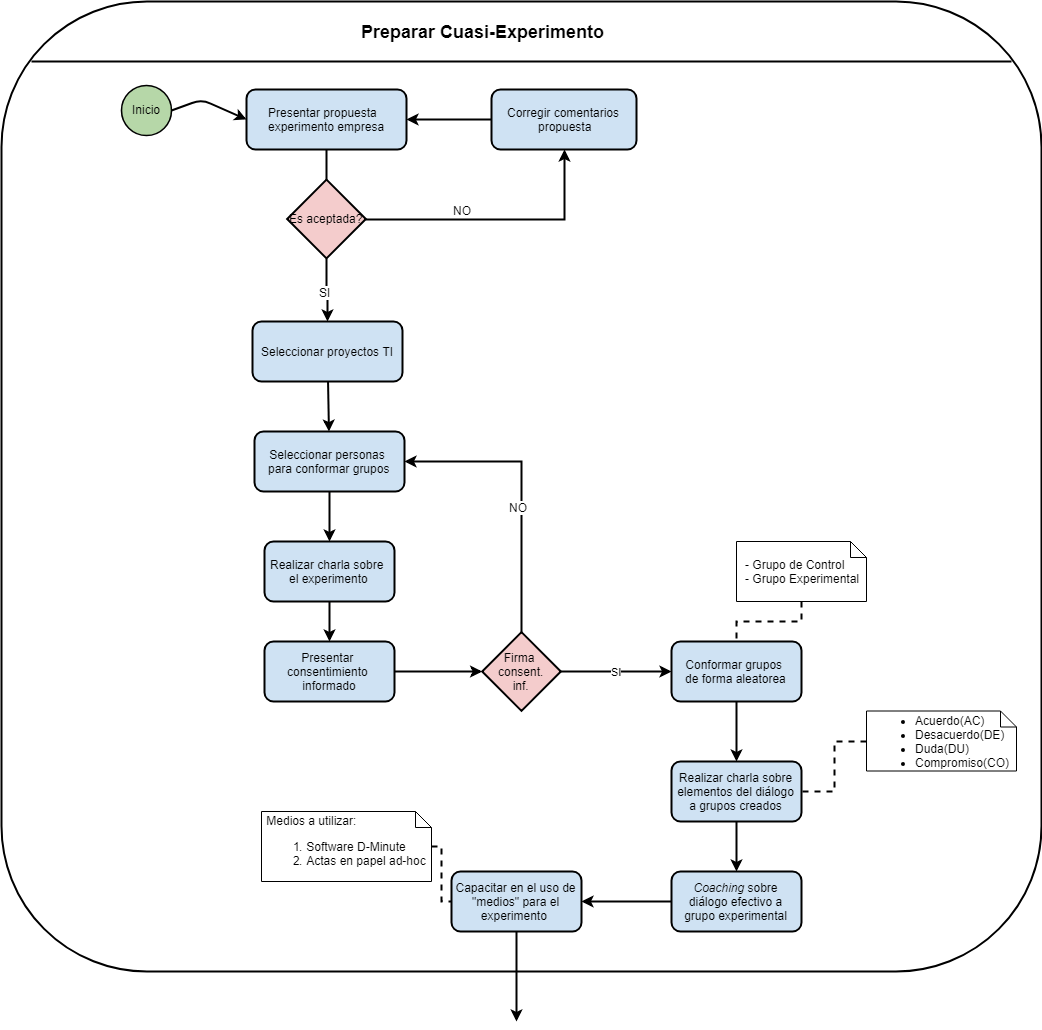
\includegraphics[width=0.8\linewidth]{/datos/recogidadatos-Page-1}
\caption{Flujo preparación del experimento,  elaboración propia} 
\label{img5-2}
\end{figure}

\begin{enumerate}[1.]
	\item Comienza con la presentación de la propuesta a la empresa, y se itera hasta su aprobación.
	\item Se seleccionan los proyectos TI que se van a evaluar.
	\item Se informa a las personas que van a participar sobre el experimento 
	\item Se informa sobre el software y la forma de interacción.
	\item Se solicita firma del consentimiento informado
	\item Se conformar grupos de control y experimental
	\item Se realiza \textit{coaching} al grupo experimental y de control.
	\item Se capacita en el uso de “medios” para realizar el experimento

\begin{figure}[!h]
\centering
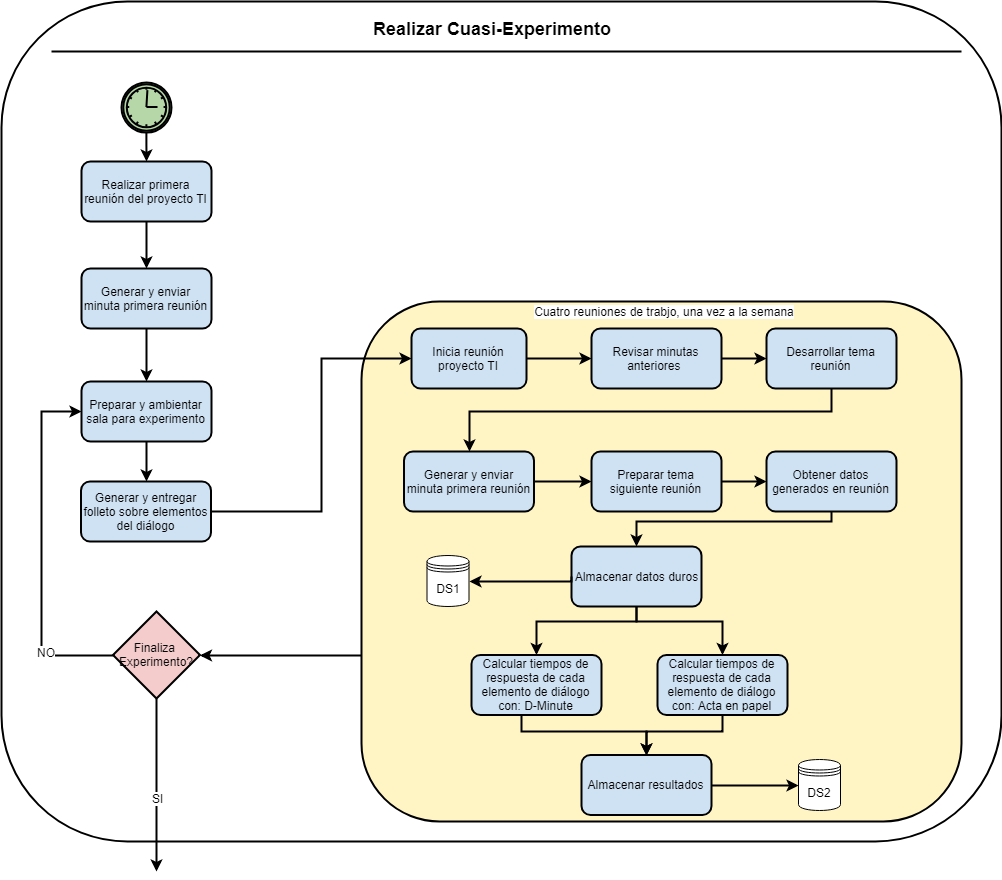
\includegraphics[width=0.8\linewidth]{/datos/recogidadatos-Page-2}
\caption{Flujo realización del experimento,  elaboración propia} 
\label{img5-3}
\end{figure}

	\item Se realiza la primera reunión del proyecto TI, la cual sirve de base para organizar las siguientes tareas del proyecto.
	\item Se prepara el ambiente para las sesiones: proyector, grabador de audio y tríptico sobre elementos del diálogo.
	\item Se inicia el experimento revisando el acta anterior y sus puntos relevantes, se ubican elementos del diálogo.
	\item Se da inicio a los siguientes temas de la reunión, se establecen los elementos del diálogo que puedan haber aparecido y se registran en el medio asignado para ello (D-Minute, actas en papel de ofimática).
	\item Se confecciona acta de la reunión y se envía a cada participante.
	\item Se almacenan los resultados y tiempos que tomó ubicar y establecer cada elemento de diálogo de los medios disponibles para el experimento.

\begin{figure}[!h]
\centering
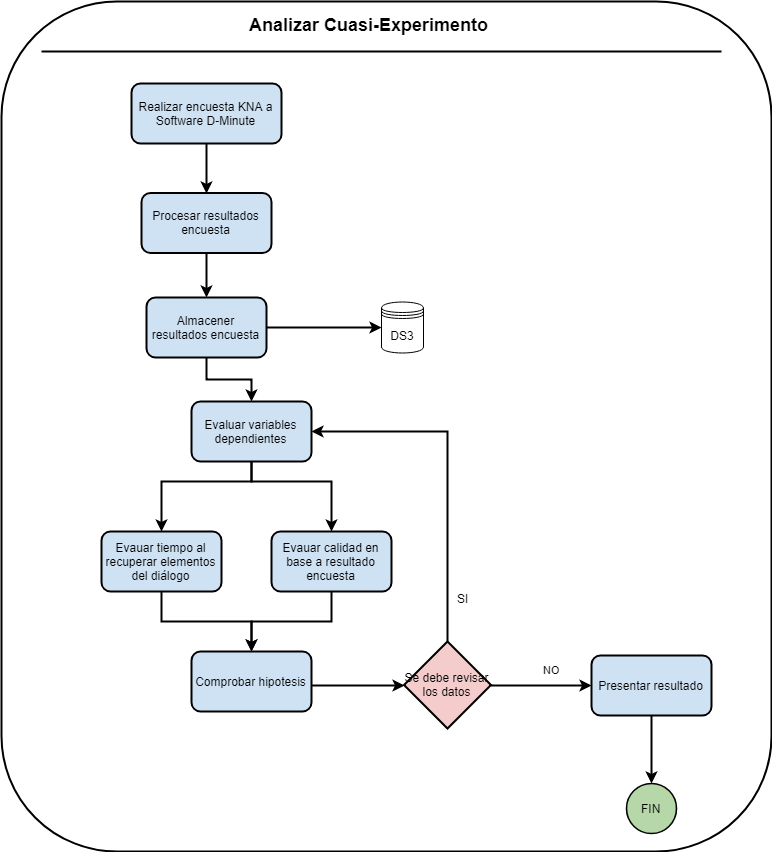
\includegraphics[width=0.8\linewidth]{/datos/recogidadatos-Page-3}
\caption{Flujo análisis del experimento,  elaboración propia} 
\label{img5-4}
\end{figure}

	\item Al finalizar las sesiones del experimento, se procede a realizar una encuesta al grupo experimental sobre la calidad del medio utilizado en el experimento.
	\item Se analizan los datos de manera no presencial y se comprueban los resultados para dar validez de las hipótesis científica.

\end{enumerate}

\subsubsection{Descripción del Dataset a ser generado}

La obtención de los datos es una de las etapas más relevantes dentro del experimento debido a que la información nos permite comprobar las hipótesis planteadas, por lo tanto se debe establecer un dataset adecuado para el conjunto de información esperado. Dado que utilizaremos instrumentos para la captura de audio y la captura de video de ambos grupos del experimento por cada reunión realizada, se propone el siguiente \textit{dataset}, ver tabla \ref{tab:dataset}.

\begin{table}[!h]
\centering
\caption{\textit{Dataset} instrumentos de reunión, elaboración propia}
\label{tab:dataset}
\resizebox{15cm}{!} {
\begin{tabular}{|l|r|l|l|l|l|}
\hline
\multicolumn{1}{|c|}{\textbf{Grupo Experimental}} & \multicolumn{1}{c|}{\textbf{Número Reunión}} & \multicolumn{1}{c|}{\textbf{Video}} & \multicolumn{1}{c|}{\textbf{Audio}} & \multicolumn{1}{c|}{\textbf{Transcripción (texto)}} & \multicolumn{1}{c|}{\textbf{Enlace Reunión (URL)}} \\ \hline
Control & 1 & reunion\_c1.mp4 & reunión\_c1.mp3 & Lorem Ipsum &  \\ \hline
Experimental & 1 & reunion\_e1.mp4 & reunión\_e1.mp3 & Lorem Ipsum &  \\ \hline
 &  &  &  &  &  \\ \hline
\end{tabular}
}
\end{table}

Para determinar nuestras hipótesis es importante determinar el tiempo que cada equipo toma en recuperar los elementos del diálogo de las reuniones pasadas y para esto se propone el siguiente dataset que nos permita recopilar la información a procesar, ver tabla \ref{tab:dataset1}.


\begin{table}[!h]
\centering
\caption{\textit{Dataset} recuperación elementos de diálogo, elaboración propia}
\label{tab:dataset1}
\resizebox{15cm}{!} {
\begin{tabular}{|l|r|l|l|r|l|}
\hline
\multicolumn{1}{|c|}{\textbf{Grupo Experimental}} & \multicolumn{1}{c|}{\textbf{Número Reunión}} & \multicolumn{1}{c|}{\textbf{Elemento de Diálogo}} & \multicolumn{1}{c|}{\textbf{Tiempo de Recuperación}} & \multicolumn{1}{c|}{\textbf{Reunión de Procedencia}} & \multicolumn{1}{c|}{\textbf{Enlace Reunión (URL)}} \\ \hline
Control & 1 & Compromiso & 5 seg. & 2 &  \\ \hline
Experimental & 1 & Duda & 15 seg. & 1 &  \\ \hline
 &  &  &  &  &  \\ \hline
\end{tabular}
}
\end{table}

Por último, si bien nuestro mayor valor es determinar el tiempo que toma cada persona en recuperar el hilo conversacional de las reuniones pasadas. Es importante determinar la circulación de conocimiento que ocurre dentro de D-Minute, para esto se requiere un dataset que nos permita recopilar las encuestas KNA (ver anexo B) aplicadas a cada sujeto que asiste a la reunión, ver tabla \ref{tab:dataset2}.

\begin{table}[!h]
\centering
\caption{\textit{Dataset} encuesta KNA para D-Minute, elaboración propia}
\label{tab:dataset2}
\resizebox{15cm}{!} {
\begin{tabular}{|l|r|l|r|l|}
\hline
\multicolumn{1}{|c|}{\textbf{Grupo Experimental}} & \multicolumn{1}{c|}{\textbf{Número Reunión}} & \multicolumn{1}{c|}{\textbf{Asistente Encuestado}} & \multicolumn{1}{c|}{\textbf{Nota Encuesta}} & \multicolumn{1}{c|}{\textbf{Enlace Reunión (URL)}} \\ \hline
Control & 1 & Oliver Hidalgo & 70 &  \\ \hline
Experimental & 1 & Juan Fuenzalida & 15 &  \\ \hline
 &  &  &  &  \\ \hline
\end{tabular}
}
\end{table}

\subsubsection{Análisis estadístico propuesto}

Para evaluar nuestras hipótesis del experimento expuesto se plantea la aplicación de diversos test estadísticos a las variables independientes descritas en las secciones anteriores. Estos test de hipótesis tendrán la finalidad de encontrar diferencias significativas en los resultados obtenidos. por tanto para determinar $\mathrm{H_{Tiempo}}$ se sugiere la aplicación de test del tipo t de student, ANOVA. Se recuerda que estos análisis son sugeridos y pueden variar al momento de definir con mayor claridad la aplicación del experimento. 

Para la circulación de conocimiento la cual es nuestra segunda hipótesis $\mathrm{H_{Conocimiento}}$, se sugiere aplicar escala de \textit{likert} a las encuestas realizadas y calcular el promedio por reunión y por grupo de control a fin de determinar nuestra hipótesis.

\subsection{RESUMEN}

El presente capítulo expuso el diseño experimental de la investigación que debe ser ejecutado para una evaluación de la herramienta D-Minute. En la primera sección se dan detalles del contexto de investigación mostrando las preguntas, variables e hipótesis que guían el estudio. Luego, la siguiente sección presenta el diseño detallado del experimento pasando por cada etapa del experimento. 

En el próximo capítulo se presentan las conclusiones del estudio presentado y los siguientes pasos.
